% ACL Rolling Review format (approximation without acl.sty)
% To finalize: replace this preamble with \usepackage{acl} once acl.sty
% is available (download from github.com/acl-org/acl-style-files).
\documentclass[11pt,twocolumn]{article}

\usepackage[utf8]{inputenc}
\usepackage[T1]{fontenc}
\usepackage{times}
\usepackage[english]{babel}
\usepackage{amsmath,amssymb}
\usepackage{graphicx}
\usepackage{booktabs}
\usepackage[hyphens]{url}
\usepackage{hyperref}
\usepackage{natbib}
\usepackage{float}
\usepackage{multirow}
\usepackage{caption}
\usepackage{subcaption}
\usepackage{colortbl}
\usepackage{xcolor}
\usepackage[letterpaper,top=1in,bottom=1in,left=1in,right=1in,
            columnsep=0.5in]{geometry}
\usepackage{microtype}
\usepackage{dblfloatfix}   % fixes figure*/table* floating too far in twocolumn
\usepackage{titlesec}
\usepackage{enumitem}

% Tighter section/subsection spacing to save vertical space
\titlespacing*{\section}{0pt}{1.2ex plus 0.3ex minus 0.2ex}{0.6ex plus 0.2ex}
\titlespacing*{\subsection}{0pt}{1.0ex plus 0.3ex minus 0.2ex}{0.4ex plus 0.2ex}
% \paragraph subtitles: italic run-in instead of bold, tighter spacing
\titleformat{\paragraph}[runin]{\normalfont\itshape}{}{0pt}{}
\titlespacing*{\paragraph}{0pt}{0.8ex plus 0.2ex}{0.5em}

% Compact lists: less indentation ("tabulation"), tighter spacing between items
\setlist[itemize]{leftmargin=1.4em, itemsep=0.1ex, topsep=0.2ex, parsep=0pt}
\setlist[enumerate]{leftmargin=1.6em, itemsep=0.1ex, topsep=0.2ex, parsep=0pt}
\setlist[description]{leftmargin=0em, itemsep=0.2ex, topsep=0.2ex, parsep=0pt}

% Allow more floats per page and reduce the threshold for placing them
\setcounter{topnumber}{4}
\setcounter{dbltopnumber}{4}
\setcounter{totalnumber}{6}
\renewcommand{\topfraction}{0.85}
\renewcommand{\dbltopfraction}{0.85}
\renewcommand{\textfraction}{0.10}
\renewcommand{\floatpagefraction}{0.80}
\renewcommand{\dblfloatpagefraction}{0.80}
\raggedbottom   % avoid stretched vertical space around headings near floats

\graphicspath{{figures/}}

\definecolor{bestrow}{RGB}{200,230,200}
\definecolor{greyrow}{RGB}{242,242,242}

\title{Biotic Interaction Detection from Scientific Literature:\\
Knowledge Distillation and Multi-task Learning\\
with Named Entity Recognition}

% ANONYMIZED FOR REVIEW
% Restore author block for camera-ready:
\author{}

\date{}

\begin{document}

\twocolumn[{%
\maketitle
\vspace{-1em}

% ─────────────────────────────────────────────────────────────────────────────
\begin{abstract}
Automated extraction of biotic interactions from scientific literature
enables large-scale knowledge graph construction over biodiversity corpora.
With Biodiversity PMC \citep{biodiversitypmc2024} alone indexing over
85\,million files, systematic manual curation is not feasible.
We present a multi-task transformer classifier combining three components:
a two-stage teacher chain in which a 122-billion-parameter local model
(Qwen3.5-122B; \citealt{qwen2025technical}) annotates $\sim$44,000 harvested sentences with binary labels and
a trained ensemble subsequently generates calibrated soft probability labels
for knowledge distillation; a multi-task BiomedBERT architecture that jointly
classifies sentences and annotates biological entities (HOST, PATHOGEN,
SPECIES, INT) using automatically derived BIO supervision; and a warm-start
initialization strategy that preserves fine-tuned encoder representations
and trains the named entity recognition (NER) head jointly from epoch one;
for this architecture and NER scheme, we find that NER pre-training epochs
are counterproductive
when task-tuned weights are reused.
On a 500-sentence multi-source test set spanning five evaluation sources,
the classifier achieves F1\,=\,0.874 (P\,=\,0.925, R\,=\,0.829; 95\% bootstrap
confidence interval (CI) [0.843, 0.902]). Relative to an identical
architecture trained with hard cross-entropy labels, the full pipeline
adds +0.202\,F1 ($p{<}0.001$, McNemar's test), of which +0.162\,F1 comes
from soft-label distillation alone (cold-start comparison). This gain is
largely calibration, not ranking: the same comparison moves the area
under the ROC curve (AUC) by only +0.024, indicating soft labels chiefly
correct the probability scale rather than the model's underlying
discrimination. The remaining +0.040\,F1 ($p{=}0.002$) comes jointly
from warm-start initialization and skipping NER pre-training --- neither
is sufficient alone (Section~\ref{sec:results}, Finding 2). The proposed
model surpasses the
BiomedBERT\,$\times$\,FLAN-T5-base ensemble teacher (F1\,=\,0.850) at
3.3$\times$ lower inference cost and is statistically indistinguishable
from the stronger single-task template-trained baseline (F1\,=\,0.875,
$p{=}0.760$) while additionally producing NER output.
On real-literature sources alone (excluding synthetic), the proposed
model leads the template-trained baseline (F1\,=\,0.847 vs.\ 0.821),
indicating the aggregate tie is driven by the synthetic subset.
The classifier is deployed upstream of
BiotXplorer \citep{sibils2023biotxplorer}, the SIBiLS \citep{mottin2021sibils}
semantic search platform for biotic interactions.
\end{abstract}

\textbf{Keywords:} biotic interactions, knowledge distillation, multi-task
learning, named entity recognition, BiomedBERT, knowledge graph,
ecological text mining, GloBI
\vspace{1em}
}]% end \twocolumn title block

% ─────────────────────────────────────────────────────────────────────────────
\section{Introduction}
\label{sec:intro}

Taxon interactions shape ecosystem structure, drive disease dynamics,
and determine the response of ecological communities to perturbation.
Cataloguing these interactions requires synthesising knowledge distributed
across millions of scientific publications.
The Global Biotic Interactions database (GloBI; \citealt{poelen2014global})
aggregates over 13\,million structured interaction records from more than 700 tabular
data sources, yet covers only a fraction of the interaction types documented
across the biodiversity literature, with 23 of 171 ROBI relation types
(ROBIext v2025, GloBI's relation ontology; \citealt{poelen2014global})
represented in our experiments.
The SIBiLS platform \citep{mottin2021sibils}, the Swiss Institute of
Bioinformatics Literature Services, provides federated semantic search over
Biodiversity PMC \citep{biodiversitypmc2024}, a curated corpus of over
85\,million biomedical and biodiversity documents encompassing both
PubMed\,Central and MEDLINE content.

Automated information extraction from scientific text has a well-established
tradition in the biomedical domain.
Named entity recognition (NER) and relation classification methods have been
applied to protein--protein interactions \citep{bunescu2005comparative},
drug--drug interactions \citep{lim2018drug}, and gene--disease associations,
with deep learning substantially improving entity detection accuracy
\citep{habibi2017deep}.
A widely used strategy for generating labelled training data at scale is
distant supervision: known interaction databases are aligned with text to
produce labels automatically, without exhaustive manual annotation
\citep{mintz2009distant}.
These approaches are predominantly designed for molecular and clinical
literature; ecological interaction types (predation, parasitism, pollination,
herbivory, mutualism) span a broader taxonomic scope and a more heterogeneous
publication landscape, with direct consequences for model generalisation
\citep{badenes2020detecting}.

A particular challenge in literature-based interaction mining is the
co-occurrence problem: a sentence may mention two organism names and an
interaction term together without actually describing an interaction between
them. Co-occurrence-based retrieval achieves high recall but suffers from
substantial false-positive rates \citep{bunescu2005comparative};
sentence-level classifiers that discriminate true interactions from
co-occurrence artefacts are a standard component of biomedical
text-mining pipelines, and the extracted triples can populate biodiversity
knowledge graphs supporting disease spread, food web, and conservation
reasoning \citep{chen2023biodiversity, poisot2021global}. Knowledge gaps
remain large, particularly for field-observed interactions published in
ecology journals outside the PubMed index \citep{poisot2021global}.

We address this gap with three primary contributions:
\begin{enumerate}
    \item A two-stage teacher chain combining large language model (LLM)
    binary annotation with ensemble-based soft probability distillation, yielding a
    44K-sentence training corpus with calibrated labels.
    \item A multi-task BiomedBERT architecture with automatic NER auxiliary
    supervision; a warm-start ablation reveals that initializing from a
    fine-tuned BiomedBERT encoder and omitting NER pre-training surpasses
    the two-phase cold-start approach (+0.040\,F1).
    \item A quantitative distribution mismatch analysis identifying the
    interaction types responsible for the current performance ceiling and
    guiding future data collection.
\end{enumerate}

% ─────────────────────────────────────────────────────────────────────────────
\section{Methods}
\label{sec:methods}

\subsection{Task Definition}

Given a sentence $s$ from scientific literature, predict $y \in \{0, 1\}$
where $y=1$ indicates that $s$ describes a biotic interaction between two
or more named organisms with the following interaction types in scope: predation, parasitism,
pathogen infection, pollination, herbivory, mutualism, symbiosis, seed
dispersal, competition, and vector-borne transmission. 
The Relation Ontology provides the conceptual framework of our study.


\subsection{Training Corpus Construction}
\label{sec:data}

\paragraph{Sentence sources.}
Two independent sentence corpora are used for different training
purposes: a synthetic template corpus that trains the single-task
baseline, and a real-literature harvested corpus that trains the
multi-task champion via knowledge distillation (Section~\ref{sec:distillation}).

\emph{Template-derived sentences (synthetic).}
Structured triples from GloBI (e.g.\ \textit{parasitizes(Anisakis simplex,
Gadus morhua)}) are injected into hand-written sentence templates covering
ten interaction categories. Every positive sentence was individually
validated by a large language model to remove formulaic or linguistically
implausible candidates, yielding 25,081 clean sentences (7,251 positive).

\emph{PMC-harvested sentences (real).}
Articles co-mentioning known GloBI taxon pairs were queried from
Biodiversity PMC \citep{biodiversitypmc2024}, both by taxon co-occurrence
and by interaction category via the SIBiLS API \citep{mottin2021sibils}.
Co-occurrence sentences were extracted and labeled by a local Qwen3.5-122B
model (a 122-billion-parameter checkpoint in the Qwen3 model family
described by \citealt{qwen2025technical})
using the prompt:
\textit{``Does this sentence describe a biotic interaction between two named
organisms? Answer yes or no only.''}
Of 44,178 harvested sentences, 4,065 (9.2\%) were accepted as positives.

\paragraph{Soft label generation.}
The accepted 44,178 sentences were re-scored by the trained BiomedBERT
$\times$ FLAN-T5-base ensemble, producing a soft probability
$p_\text{ensemble} \in [0,1]$ per sentence. These soft labels constitute
the distillation teacher signal (Section~\ref{sec:distillation}).

\subsection{Model Architecture Evolution}
\label{sec:architectures}

Our experiments are split and evaluated using five distinct steps with an increasing order of
complexity.

\paragraph{Classical baselines.}
A support vector machine (SVM) and Random Forest on term frequency-inverse
document frequency (TF-IDF) features achieved F1\,$\approx$\,0.62,
establishing the need for contextual representations.

\paragraph{Template-trained BiomedBERT.}
We use the BiomedBERT model \citep{gu2021domain}
(\url{microsoft/BiomedNLP-BiomedBERT-base-uncased-abstract-fulltext}),
a BERT-base model (110M parameters, 12 transformer
layers, 768-dimensional hidden states) pre-trained from scratch on PubMed
abstracts and PubMed Central full-text articles. A linear classification
head on the [CLS] token representation is fine-tuned using 5-fold
cross-validation, AdamW optimiser ($\eta = 2 \times 10^{-5}$, weight
decay\,=\,0.01), and threshold optimisation on the validation split.

All subsequent models (ensemble, distilled student, multi-task champion)
use this same BiomedBERT encoder and differ only in training objective or
auxiliary supervision. This baseline (Table~\ref{tab:main_results}, row 6)
is trained on template-generated training data via standard
cross-entropy and achieves F1\,=\,0.875 on the 500-sentence test set.
Its strong aggregate performance masks divergent per-source behaviour
(Figure~\ref{fig:version_f1}), discussed in detail in
Section~\ref{sec:reversal}: neither this baseline nor the multi-task
warm-start champion (Section~\ref{sec:multitask}) dominates uniformly
across all five test sources.
This model also acts as the BiomedBERT component of the teacher ensemble
described below.

\begin{figure*}[!ht]
    \centering
    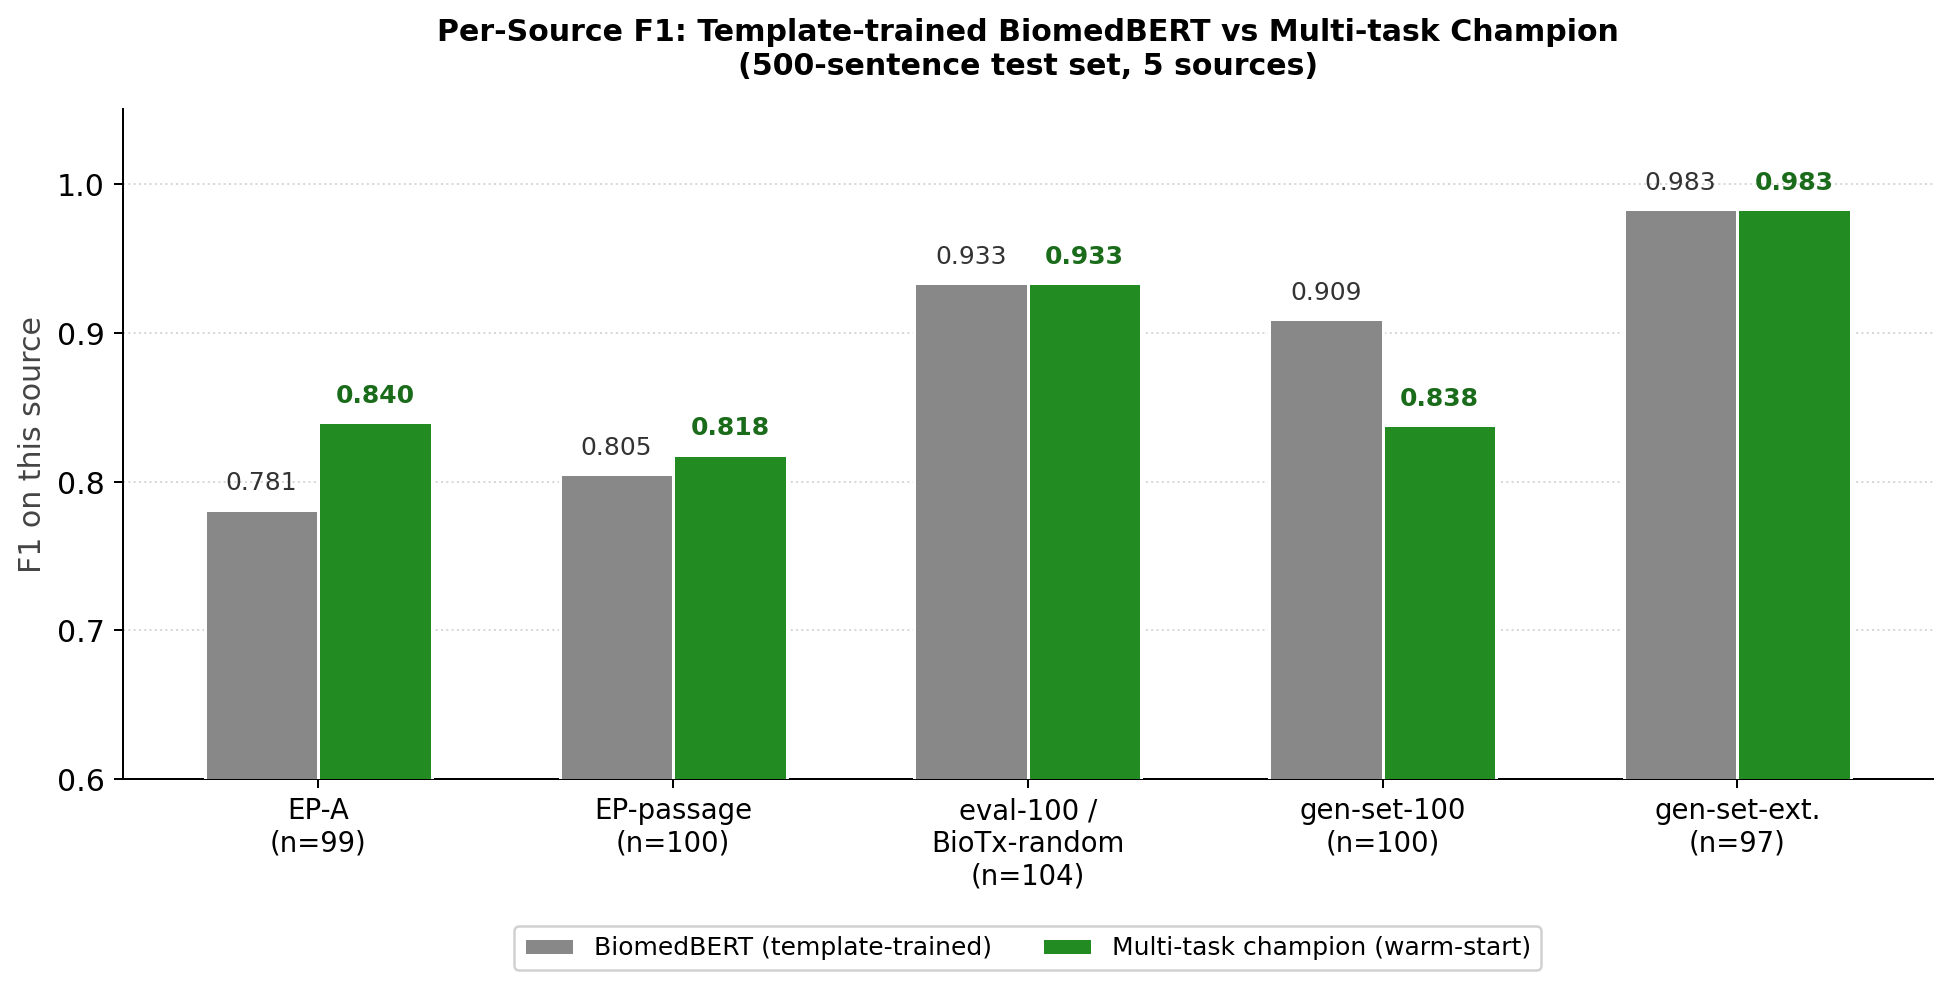
\includegraphics[width=0.8\textwidth]{fig_01_version_f1}
    \caption{Per-source F1 comparing the template-trained BiomedBERT baseline
    against the multi-task warm-start champion (Section~\ref{sec:multitask}).
    Per-source $n$ shown on the $x$-axis; ``gen-set-ext.'' is
    gen-set-150-extension (Section~\ref{sec:eval}), 97 sentences kept after
    independent gold-label validation out of 150 drafted.}
    \label{fig:version_f1}
\end{figure*}

\paragraph{BiomedBERT\,$\times$\,FLAN-T5-base ensemble.}
FLAN-T5-base \citep{chung2022scaling}, a sequence-to-sequence model trained
with instruction tuning, was fine-tuned as a binary classifier by prompting
for a yes/no answer and scoring the first generated token. The geometric
mean of BiomedBERT and FLAN-T5-base predicted probabilities, with joint
threshold optimisation, achieves F1\,=\,0.850 on the 500-sentence test set.
The gain over a single model is attributable to model complementarity:
BiomedBERT handles precise, template-like language while FLAN-T5-base
generalises better to paraphrased ecological sentences.

The two subsequent stages, knowledge distillation and multi-task NER, are
described in Sections~\ref{sec:distillation} and~\ref{sec:multitask}
respectively. Figure~\ref{fig:model_evolution} (Appendix~\ref{app:extended_discussion})
summarises the F1 progression across architecture stages shown numerically
in Table~\ref{tab:main_results}.

\subsection{Knowledge Distillation}
\label{sec:distillation}

Knowledge distillation \citep{hinton2015distilling} transfers calibrated
uncertainty from a teacher to a student by training on soft probability
distributions rather than hard labels \citep{bucilua2006model}, which is
especially valuable for borderline sentences.

\paragraph{Training objective.}
The student BiomedBERT is trained using Kullback-Leibler (KL) divergence
against the ensemble teacher:
\begin{equation}
    \mathcal{L}_\text{KL} = T^2 \cdot \mathrm{KL}\!\left(
        \sigma(\mathbf{z}_s / T) \;\|\; \sigma(\mathbf{z}_t / T)
    \right)
\end{equation}
where $T$ is the temperature, $\mathbf{z}_s$ and $\mathbf{z}_t$ are student
and teacher logits, and $\sigma$ denotes the softmax function.
Rows without soft labels use hard cross-entropy. The combined loss is
$\mathcal{L} = \alpha \cdot \mathcal{L}_\text{KL} + (1{-}\alpha) \cdot \mathcal{L}_\text{CE}$.

Optimal hyperparameters ($T{=}2$, $\alpha{=}0.5$) were identified by
grid search over six student configurations (Appendix~\ref{app:distillation}).
Temperature $T{=}2$ spreads the teacher distribution sufficiently to
transfer calibrated uncertainty without over-smoothing; it also corrects
for ensemble overconfidence at $p{>}0.9$ (expected calibration error,
ECE\,=\,0.148 on EP-A),
where the ensemble's mean confidence of 0.967 exceeds its accuracy of 0.804. The best-performing
student achieves F1\,=\,0.858 on the 500-sentence test set.

\subsection{Multi-task BiomedBERT with NER Auxiliary Task}
\label{sec:multitask}

\paragraph{Architecture.}
The BiomedBERT encoder is extended with two linear output heads that share
all encoder weights:
\begin{itemize}
    \item \textit{Classification head}: reads the [CLS] token vector
    ($\mathbb{R}^{768} \to \mathbb{R}^2$), produces $P(\text{interaction})$.
    \item \textit{NER head}: reads every token vector
    ($\mathbb{R}^{768} \to \mathbb{R}^{|\mathcal{L}|}$), produces
    Beginning-Inside-Outside (BIO; \citealt{ramshaw1995text}) tagging-scheme
    label logits.
\end{itemize}

\paragraph{NER label scheme.}
We index $\approx$4.2\,million binomial taxon names plus 21K common
names into a gazetteer, matched against text via Aho-Corasick automata
\citep{aho1975efficient} for exact string lookup.

We use the \texttt{full\_typed} scheme with $|\mathcal{L}| = 9$ labels:
\texttt{O} (background), \texttt{B/I-HOST} (hosting organism),
\texttt{B/I-PATHOGEN} (infecting or parasitic agent),
\texttt{B/I-SPECIES} (ambiguous role in symmetric interactions),
\texttt{B/I-INT} (interaction verb or phrase).
In addition to taxon gazetteers, labeling relies on an interaction lexicon
developed within SIBiLS \citep{mottin2021sibils}, containing 591 terms derived
from the GloBI relation ontology (ROBI), covering all interaction types indexed
by BiotXplorer, supplemented by 50 biomedical terms for pathogen-host vocabulary
not represented in ROBI.
Gold taxon annotations from training metadata override gazetteer lookup when
available.

Table~\ref{tab:ner_schemes} compares the four label schemes evaluated.
The HOST/PATHOGEN distinction encodes the direction of the relation: who acts
and who is acted upon. This directional labelling is motivated by the downstream
knowledge graph construction task, where edge direction is semantically significant.

\begin{table*}[!ht]
\centering
\small
\caption{NER label schemes compared in the configuration analysis
(Section~\ref{sec:results}). B\,=\,beginning, I\,=\,inside span.
F1 is the best \emph{cold-start} result for that scheme, for a like-for-like
comparison (full ablation in Appendix~\ref{app:fullablation}). \texttt{full\_typed}
lacks the highest cold-start F1 but is carried forward to the warm-start
ablation (0.874, Table~\ref{tab:main_results}) for its HOST/PATHOGEN typing
(Section~\ref{sec:zerocost}).}
\label{tab:ner_schemes}
\begin{tabular}{lclr}
\toprule
\textbf{Scheme} & \textbf{\# labels} & \textbf{Label set} & \textbf{F1} \\
\midrule
\rowcolor{bestrow}
\textbf{basic}       & \textbf{3} & \textbf{O,\ B/I-SPECIES}                            & \textbf{0.861} \\
\texttt{typed}       & 5 & O,\ B/I-HOST,\ B/I-PATHOGEN                         & 0.794 \\
\texttt{full}        & 5 & O,\ B/I-SPECIES,\ B/I-INT                           & 0.858 \\
\texttt{full\_typed} & 9 & O,\ B/I-HOST,\ B/I-PATHOGEN,\ B/I-SPECIES,\ B/I-INT & 0.840 \\
\bottomrule
\end{tabular}
\end{table*}

\paragraph{Training strategy.}
We compare two initialization strategies.

\emph{Cold-start (two-phase).}
When initializing from general pretrained BiomedBERT weights, training
proceeds in two phases designed to avoid interference between the NER and
classification objectives \citep{liu2019multi}:
\begin{description}
    \item[Phase 1: NER pre-train ($E_\text{NER}$ epochs).]
    The classification head is frozen. Only the encoder and NER head receive
    gradient updates from token-level cross-entropy loss
    $\mathcal{L}_\text{NER}$.
    This phase primes the shared encoder to locate taxon names and
    interaction verbs before the classification signal is introduced.

    \item[Phase 2: Joint training ($E_\text{joint}$ epochs).]
    All parameters are unfrozen. Combined loss:
    \[
        \mathcal{L} = \alpha \cdot \mathcal{L}_\text{cls} +
                      (1{-}\alpha) \cdot \mathcal{L}_\text{NER}
    \]
    where $\mathcal{L}_\text{cls}$ is soft KL divergence against ensemble
    soft labels when available, and hard CE otherwise.
\end{description}
With $E_\text{NER}{=}2$ and $E_\text{joint}{=}3$, this achieves
F1\,=\,0.835 (Table~\ref{tab:main_results}, row 2).

\emph{Warm-start (proposed champion).}
We initialize the BiomedBERT encoder from the Template-trained
BiomedBERT classification checkpoint and skip Phase 1 entirely: both the NER head and
the classification head train jointly from epoch one.
This strategy achieves F1\,=\,0.874 at $\tau{=}0.360$, the best result in our evaluation.
Ablation over the number of NER pre-training epochs under warm-start
reveals a clear negative correlation (Appendix~\ref{app:fullablation},
warm-start rows): F1\,=\,0.874 with 0 NER epochs, 0.860 with 1, and
0.822 with 2.
We attribute this to \emph{representation disruption}: the template-trained
BiomedBERT encoder already encodes biotic interaction patterns from classification
fine-tuning; NER pre-training updates the shared encoder toward
entity-detection representations, degrading the classification-relevant
signal. Warm-starting without Phase 1 preserves this initialization
while the NER head still learns entity recognition through the joint
objective in Phase 2.

\subsection{Evaluation Protocol}
\label{sec:eval}

All models are evaluated on a 500-sentence test set (281 positive,
56.2\%) combining five sources: EP-A (99 sentences, GloBI-seeded),
EP-passage (100 sentences, GloBI-seeded), a merged eval-100/BioTx-random
source (104 sentences), gen-set-100 (100 synthetic sentences), and
gen-set-150-extension (97 additional synthetic sentences added to
restore the test set to 500). Source construction, deduplication, and
the independent gold-label validation of gen-set-150-extension are
detailed in Section~\ref{sec:contamination} and
Appendix~\ref{app:contamination}.
We report precision, recall, and F1-score.
The decision threshold $\tau$ is optimised on the validation split,
not the test set. For the warm-start champion, $\tau = 0.360$ is derived
from the standard 15\% held-out split of its training data. For the
cold-start ablation, $\tau = 0.140$ is derived from the same kind of split;
this lower value reflects the cold-start model's probability
distribution skewing toward lower scores (Appendix~\ref{app:threshold}).

Bootstrap confidence intervals are estimated with 10,000 resamples
\citep{efron1993introduction}.
Pairwise significance is assessed using McNemar's test
\citep{mcnemar1947note} with continuity correction.

\subsection{Test Set Integrity}
\label{sec:contamination}

We ran three checks (exact-match, near-duplicate, taxon-pair leakage,
Appendix~\ref{app:contamination}) between the test set and every
training corpus used to produce a reported model. These checks confirm
the test set is independent of the training data used to produce every
reported result, with one exception: exactly one test sentence (from a
SIBiLS-harvested source) also appears in a broader corpus not used to
train any reported model. The same procedure uncovered that the
eval-100 and BioTx-random sources, nominally independent, share 96 of
100 sentences as the same underlying content exported in two formats;
they are merged into a single deduplicated source (Section~\ref{sec:eval}).
The checks cannot rule out overlap with BiomedBERT's own pretraining
corpus (PubMed abstracts and full-text articles,
\citealt{gu2021domain}), since several test sources are themselves
drawn from PMC and we have no access to that corpus to verify this
either way. A related gold-label provenance caveat, distinct from
sentence-level leakage, is discussed in Section~\ref{sec:limitations}.

\begin{table*}[!t]
\centering
\small
\caption{Main results on the 500-sentence test set (281 positives).
The proposed warm-start multi-task model (top, \textbf{champion}) significantly outperforms the
hard-CE ablation ($+0.202$ F1, $p{<}0.001$) and surpasses the ensemble teacher
at 3.3$\times$ lower inference cost (a single BiomedBERT forward pass versus
the ensemble's additional FLAN-T5-base sequence-to-sequence decoding step).
Full configuration sweep in Appendix~\ref{app:fullablation}. F1 values are
rounded to three decimals for display; reported deltas and significance
tests use unrounded scores, so pairwise differences may not equal the
difference of displayed values.}
\label{tab:main_results}
\begin{tabular}{lrrrr}
\toprule
\textbf{Model} & \textbf{F1} & \textbf{P} & \textbf{R} & \textbf{AUC} \\
\midrule
\rowcolor{bestrow}
\textbf{Multi-task BiomedBERT} (\texttt{full\_typed}, $\alpha$=0.5, warm-start, 0 NER ep) & \textbf{0.874} & \textbf{0.925} & \textbf{0.829} & \textbf{0.918} \\
\midrule
\rowcolor{greyrow}
Multi-task BiomedBERT (\texttt{full\_typed}, $\alpha$=0.5, cold-start, 2 NER ep) & 0.835 & 0.885 & 0.790 & 0.881 \\
\rowcolor{greyrow}
Same arch., hard cross-entropy (no distillation)    & 0.673 & 0.920 & 0.530 & 0.857 \\
\rowcolor{greyrow}
Distilled student (BiomedBERT, $T$=2, $\alpha$=0.5) & 0.858 & 0.877 & 0.840 & 0.920 \\
\rowcolor{greyrow}
Ensemble BiomedBERT $\times$ FLAN-T5-base           & 0.850 & 0.925 & 0.787 & 0.912 \\
\rowcolor{greyrow}
Template-trained BiomedBERT (single-task baseline)  & 0.875 & 0.881 & 0.868 & 0.921 \\
\bottomrule
\end{tabular}
\end{table*}

% ─────────────────────────────────────────────────────────────────────────────
\section{Results}
\label{sec:results}

\subsection{Multi-task Configuration Analysis}

Table~\ref{tab:main_results} compares the champion configuration against
key baselines; the full sweep over all NER schemes, $\alpha$ values,
initialization strategies, and pre-training epochs is given in
Appendix~\ref{app:fullablation}. AUC, reported alongside F1/P/R as a
threshold-independent measure of ranking quality, broadly agrees with
the F1 picture: the champion, template-trained baseline, distilled
student, and ensemble form a tight cluster (AUC 0.912--0.921) with
overlapping discriminative power, while hard-CE trails (0.857).
Notably, hard-CE's AUC gap to this cluster (0.055--0.064) is much
smaller than its F1 gap (0.177--0.202), consistent with the calibration
argument in Section~\ref{sec:distillation}: hard-CE's underlying ranking
ability is closer to the soft-label models than its F1 alone suggests,
and its larger weakness is poor probability calibration at the
operating threshold.

Four consistent findings emerge from the analysis:

\paragraph{1. Soft labels are the largest single lever (+0.162 F1).}
The \texttt{hardce} configuration is architecturally identical to the
cold-start champion (\texttt{full\_typed} scheme, $\alpha{=}0.5$,
2 NER pre-training epochs, cold-start) and differs only in the
classification loss (hard cross-entropy instead of soft-KL), achieving
F1\,=\,0.673. The soft-KL variant (cold-start multi-task) reaches 0.835:
a difference of +0.162 F1 ($p{<}0.001$, McNemar's test) attributable
purely to the loss function, larger than any architectural change.
The further +0.040 F1 to reach the warm-start champion (0.874) is a
separate, architectural effect (warm-start initialization with zero
NER pre-training epochs), isolated in Finding 4 below.

\paragraph{2. NER pre-training epochs matter only under warm-start.}
Under cold-start, 0 and 2 NER pre-training epochs are statistically
indistinguishable (0.840 vs.\ 0.835). Under warm-start, the picture is
unambiguous: adding epochs \emph{hurts} (0 ep: 0.874 $>$ 1 ep: 0.860 $>$
2 ep: 0.822). NER pre-training disrupts the fine-tuned encoder's
classification representations when they already exist; with no such
representations under cold-start, epoch count matters far less.

\paragraph{3. NER scheme richness alone does not predict cold-start performance.}
Under cold-start (all four schemes trained on identical data), there is no
monotonic trend by label-set size: \texttt{basic} (0.861) and \texttt{full}
(0.858) outperform \texttt{full\_typed} (0.840), while \texttt{typed} (0.794),
HOST/PATHOGEN-only, is weakest of all. \texttt{full\_typed}'s advantage
materializes only with warm-start (Finding 4), reaching 0.874, the highest
result overall; we retain it regardless because its HOST/PATHOGEN typing is
required for the downstream knowledge-graph use case (Section~\ref{sec:zerocost}).

\paragraph{4. Warm-start initialization closes the gap with the template-trained baseline.}
Initializing from the template-trained BiomedBERT checkpoint and skipping NER
pre-training achieves F1\,=\,0.874, an improvement of +0.040 over the
cold-start champion (0.835). The gap with the template-trained single-task
model (F1\,=\,0.875) is 0.0003 and is not statistically significant
(Section~\ref{sec:stats}). The warm-start champion additionally produces NER
labels at no extra inference cost.

\subsection{Statistical Significance}
\label{sec:stats}

McNemar's test \citep{mcnemar1947note} is appropriate for this comparison
because predictions are binary (correct or incorrect per sentence), the
models are evaluated on the same test examples (paired observations), and
the test specifically targets prediction disagreements rather than assuming
a continuous performance metric. Under the null hypothesis that two models
commit errors on the same sentences, the reported $p$-value is the probability
of observing prediction disagreements as extreme as those measured.

Figure~\ref{fig:ci} shows 95\% bootstrap confidence intervals on the
500-sentence test set.

\begin{figure}[!ht]
    \centering
    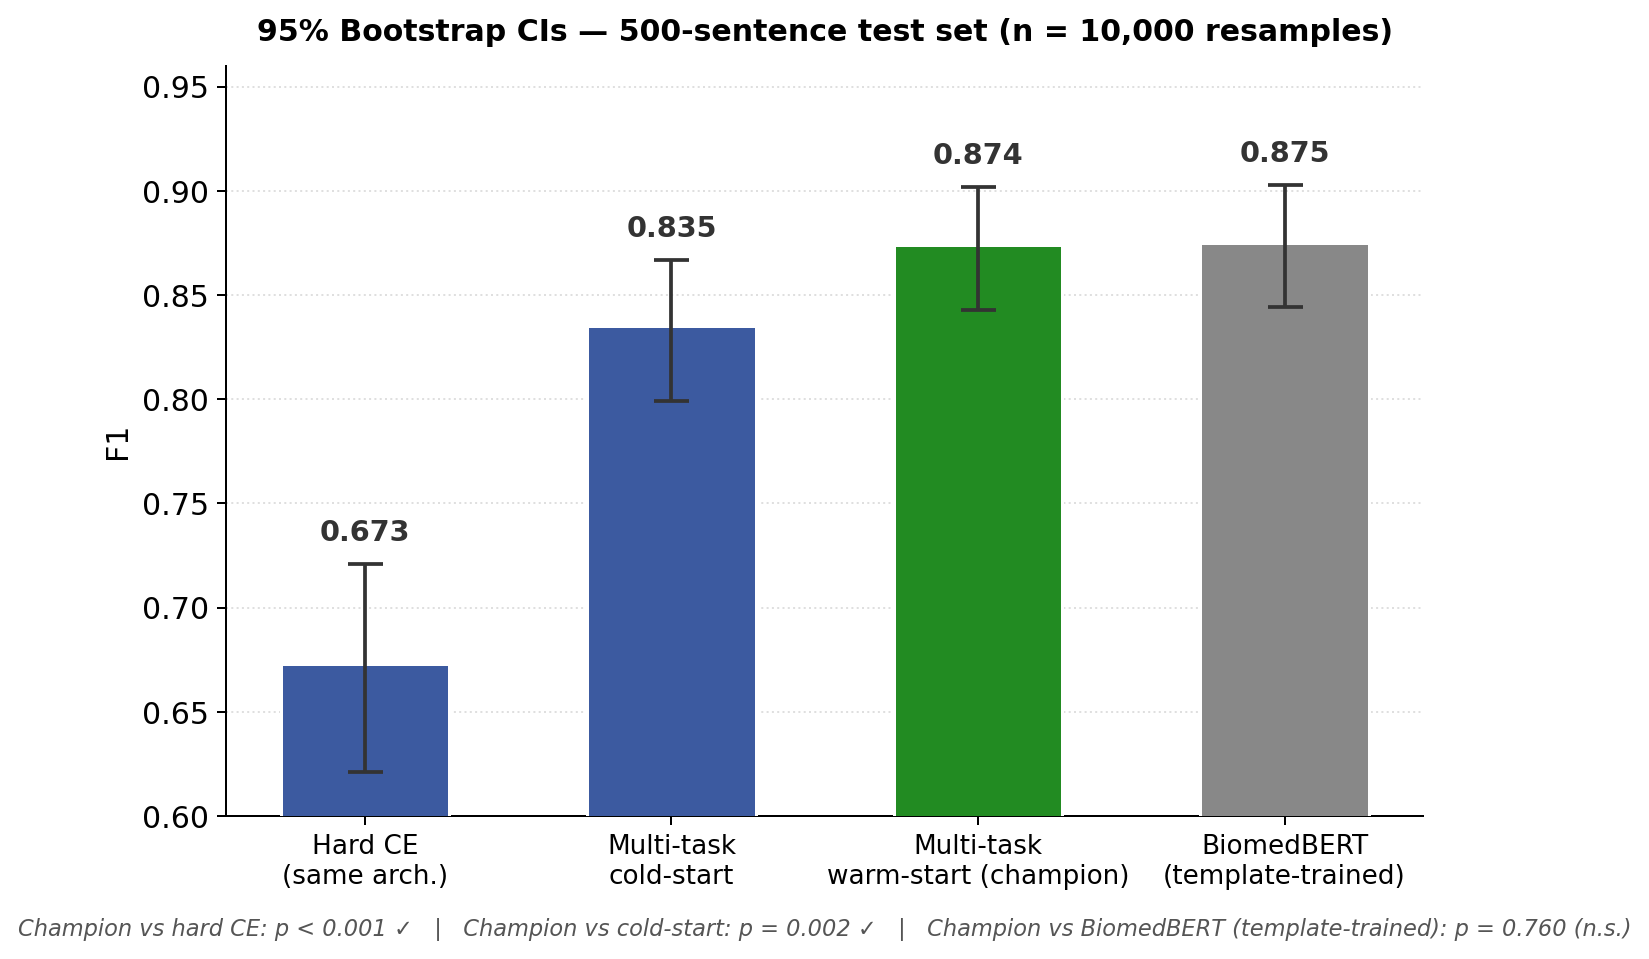
\includegraphics[width=\columnwidth]{fig_manuscript_ci}
    \caption{Bootstrap 95\% confidence intervals for four models on the
    500-sentence test set. Significance annotations refer to McNemar's test.}
    \label{fig:ci}
\end{figure}

The warm-start champion significantly outperforms the hard cross-entropy
baseline ($p{<}0.001$): 113 sentences correctly classified by the champion
but not by hard CE, versus 35 in the reverse direction (+0.202\,F1).
It also significantly outperforms the cold-start multi-task model
($p{=}0.002$): 32 sentences correctly classified by warm-start
but not by cold-start, versus 11 in the reverse direction (+0.040\,F1).
Compared with the single-task template-trained baseline (F1\,=\,0.875),
the champion's deficit is 0.0003\,F1 and is not statistically significant
($p = 0.760$, 23 vs.\ 20 disagree in each direction): the multi-task warm-start model
is statistically indistinguishable from the template-trained baseline while
additionally providing NER output. By contrast, the cold-start multi-task
model is significantly weaker than the template-trained baseline
($p{=}0.045$), underscoring that warm-start initialization, not the
multi-task architecture alone, is what closes this gap.
The 95\% bootstrap CIs for the champion [$0.843, 0.902$] and the
template-trained baseline [$0.844, 0.903$] overlap substantially, confirming
reliable model selection between them is not possible at this test set size
(see also Section~\ref{sec:limitations}).

Threshold sensitivity and operating-point trade-offs are analysed in
Appendix~\ref{app:threshold}.

\subsection{Distribution Mismatch}

The training corpus, harvested via the SIBiLS API,
is dominated by predation (42\%), herbivory (22\%), and pollination (22\%)
sentences.
Parasitism/Host interactions represent only 10\% of training positives, and
Pathogen/Infection only 3\%, yet together these two types constitute 68\%
of test positives (Parasitism/Host 41.6\%, Pathogen/Infection 26.3\%),
visualised in Figure~\ref{fig:distribution} (Appendix~\ref{app:extended_discussion}).

This mismatch reflects a structural property of the harvested corpus:
clinical and biomedical pathogen papers dominate its open-access content,
while field-observed host-parasite interactions remain underrepresented.
The full 500-sentence test set spans five annotation sources
with diverse interaction-type distributions, including synthetic sentences
covering all ten in-scope categories (gen-set-100). The distributional gap
between training and test is expected: it identifies where to invest in
future data collection to improve robustness across interaction types.

% ─────────────────────────────────────────────────────────────────────────────
\section{Discussion}
\label{sec:discussion}

\subsection{Soft Labels as the Primary Driver of Improvement}

The soft-label and warm-start gains quantified in
Section~\ref{sec:results} (Finding 1) are consistent with the knowledge
distillation literature \citep{hinton2015distilling, tang2019distilling}:
a teacher exposed to diverse linguistic expressions of interactions
assigns calibrated probabilities to borderline sentences, encoding
semantic uncertainty hard labels cannot represent. This is a calibration
mechanism rather than a ranking improvement (Section~\ref{sec:results}):
soft labels act mainly on \emph{where} the decision boundary falls, not
on the model's ability to separate positives from negatives.

\subsection{Matching Template-Trained Performance via Warm-Start}
\label{sec:reversal}

The warm-start multi-task champion is statistically
indistinguishable from the template-trained baseline
(Section~\ref{sec:stats}).
Figure~\ref{fig:version_f1} breaks this aggregate equivalence down by
test source: the champion is more competitive on the two GloBI-seeded
passage sources (EP-A: 0.840 vs.\ 0.781; EP-passage: 0.818 vs.\ 0.805),
the template-trained baseline is stronger on gen-set-100 (0.909 vs.\
0.838), and the two models are within 0.001\,F1 of each other on the
eval-100/BioTx-random and gen-set-150-extension sources. The aggregate
tie is therefore not a uniform tie at the source level, but two models
with complementary strengths reaching the same overall score.

Grouping by provenance sharpens this further: the champion
leads on the 303 real-literature sentences (directional, $p{=}0.067$),
while the template-trained baseline leads on the 197 synthetic sentences
(0.946 vs.\,0.913) --- the aggregate tie is the net of two opposing
effects, not genuine equivalence.

By contrast, the cold-start champion (F1\,=\,0.835) is nominally weaker
than the template-trained baseline ($p{=}0.045$); with five comparisons
reported here, this would not survive a Bonferroni correction
($\alpha{=}0.01$), so we treat it as suggestive only.
The key difference is that cold-start training on the 44K corpus
displaces the template-aligned representations built during template
pretraining, whereas warm-start retains them. The warm-start champion
additionally outputs NER labels (HOST, PATHOGEN, SPECIES, INT, Finding 4),
unlike the template-trained baseline's binary-only output.

\subsection{NER as Zero-Cost Auxiliary Supervision}
\label{sec:zerocost}

The NER auxiliary task improves classification without additional manual
annotation: BIO labels \citep{ramshaw1995text} come from taxon gazetteers
and interaction lexicons (distant supervision, \citealt{mintz2009distant}),
and the NER head produces entity labels at inference time at no extra
cost. The HOST/PATHOGEN distinction it outputs directly encodes
knowledge-graph edge direction, benefiting both BiotXplorer's
search ranking and downstream relation extraction. Extended discussion
of the mechanism and concrete operational use cases is given in
Appendix~\ref{app:extended_discussion}.

\subsection{The Training Distribution Ceiling}

Given that the architecture-level gap with the template-trained baseline is
already closed (Section~\ref{sec:reversal}), and the training/test
distribution mismatch identified in Section~\ref{sec:results} is large
relative to it, further improvement is more likely to come from
expanding the training corpus's coverage of parasitism/host and
pathogen/infection interactions than from further architectural changes.

\subsection{Limitations}
\label{sec:limitations}

\begin{enumerate}
    \item \textit{Teacher chain dependence.} The soft-label ensemble was
    trained on template-derived and early PMC-harvest data (pre-Qwen), so
    Qwen3.5-122B and the ensemble are orthogonal signal sources; overlap
    with the template baseline's training data is zero, and only 5.1\% of
    distillation sentences appear elsewhere in the corpus (predominantly
    low-confidence negatives, mean $p_\text{ensemble}=0.20$). Soft labels
    are also imperfectly calibrated (Section~\ref{sec:distillation}). The
    same dependence touches test-gold validation: gen-set-150-extension's
    labels were validated by the same Qwen3.5-122B model that generates
    every training label, sharing a common annotator bias for that source.
    EP-A is human-curated and independent of both teachers, our clean
    anchor against this risk.

    \item \textit{Test set composition.} The 500-sentence test set combines
    five sources, two synthetic (gen-set-100, gen-set-150-extension). No
    single style uniformly favours either model (Section~\ref{sec:reversal}).
    95\% CIs span $\pm$0.030 F1. Marginal CIs overlap for the champion--baseline pair, so they cannot be separated on F1 alone; the paired McNemar test still resolves the larger pairwise gaps reliably (Section~\ref{sec:stats}).

    \item \textit{Binary classification.} The classifier detects interactions
    but does not classify interaction type. Downstream relation extraction
    is needed to produce typed knowledge graph edges.

    \item \textit{NER head not directly evaluated.} We evaluate the NER
    head only through its effect on classification; direct entity-span
    evaluation (HOST/PATHOGEN/SPECIES/INT) against manually curated gold is
    left to future work, as the distant-supervision labels share the
    gazetteer's blind spots and cannot serve as an independent gold
    standard.

    \item \textit{English only.} Training and evaluation are exclusively
    English-language.
\end{enumerate}

% ─────────────────────────────────────────────────────────────────────────────
\section{Conclusion}

We have presented a multi-task BiomedBERT classifier for sentence-level
biotic interaction detection that achieves F1\,=\,0.874 (P\,=\,0.925,
R\,=\,0.829) on a 500-sentence multi-source test set. The model is built
on three components: a two-stage teacher chain combining large-LLM binary
annotation with ensemble soft-probability distillation over 44K sentences;
a multi-task NER auxiliary task with automatic BIO supervision from taxon
gazetteers; and a warm-start initialization from a fine-tuned BiomedBERT
encoder that trains the NER head jointly from epoch one.

The central quantitative findings are: (1) soft-label distillation is the
largest single lever, contributing +0.162\,F1 over hard cross-entropy on
identical architecture and data ($p{<}0.001$), though the matching AUC
change of +0.024 shows this gain is predominantly improved calibration
at the operating threshold rather than better ranking; (2) warm-start
initialization combined with skipping NER pre-training adds a further
+0.040\,F1 ($p{=}0.002$) --- neither component suffices alone ---
bringing the total gain over hard CE to +0.202\,F1; and (3) the
warm-start multi-task model is statistically indistinguishable from the
template-trained baseline (F1\,=\,0.875, $p{=}0.760$) while surpassing
the ensemble teacher (F1\,=\,0.850) at 3.3$\times$ lower inference cost
and additionally providing NER output for downstream knowledge graph
construction.

The classifier is deployed in BiotXplorer
(\url{https://biotxplorer.sibils.org/}) as an upstream quality filter
and constitutes the first component of a knowledge graph construction
pipeline for biodiversity and host-pathogen interactions. Future work
will address: (1) harvesting from non-PubMed ecological literature to
expand training coverage of parasitism and host-interaction types;
(2) typed relation extraction to produce directed knowledge graph triples;
(3) integration with amplicon sequencing pipelines (MetaPlantCode project;
\citealt{gardette2024metaplantcode}),
where interaction knowledge can support ecological coherence re-ranking of
taxon lists derived from environmental DNA samples.

% ─────────────────────────────────────────────────────────────────────────────
\section*{Ethics Statement}

This work raises no ethical concerns. Training data consists of sentences
automatically extracted from open-access scientific literature and labeled
by automated models; no personal data was collected or used. The classifier
is designed to support literature mining for biodiversity knowledge graph
construction and carries no foreseeable potential for misuse.

\section*{Data and Code Availability}

Training code, evaluation scripts, and the test set are available at
\url{https://anonymous.4open.science/r/biotic-interaction-classifier-anon-28DC}.
Model weights can be reproduced from the provided training configuration.

\bibliographystyle{abbrvnat}
\bibliography{references}

% ─────────────────────────────────────────────────────────────────────────────
\clearpage
\onecolumn
\appendix

\section{Knowledge Distillation Hyperparameter Search}
\label{app:distillation}

\begin{table}[H]
\centering
\caption{Full distillation hyperparameter grid on the 500-sentence test set
(281 positives). These are single-task distilled classifiers (no NER head,
not the multi-task architecture used elsewhere in this paper), so their
calibration and threshold $\tau{=}0.25$ (training-split-derived) are independent
of, and not comparable to, the multi-task champion's $\tau{=}0.360$ or the
cold-start ablation's $\tau{=}0.140$.
All variants use BiomedBERT as student except v4 (DistilBERT)
and v5 (SciBERT). Rows marked $^{\ddagger}$ use checkpoints no longer
available for re-evaluation on the current test set version; their values
are retained from a prior test-set version for completeness.}
\label{tab:distillation_full}
\begin{tabular}{lccc}
\toprule
\textbf{Student} & $T$ & $\alpha$ & \textbf{Test F1} \\
\midrule
v1 BiomedBERT & 4 & 0.7 & 0.851 \\
\rowcolor{bestrow}
\textbf{v2 BiomedBERT (best)} & \textbf{2} & \textbf{0.5} & \textbf{0.858} \\
v3 BiomedBERT$^{\ddagger}$ & 4 & 0.9 & 0.704$^{\dagger}$ \\
v4 DistilBERT$^{\ddagger}$ & 2 & 0.5 & 0.785 \\
v5 SciBERT$^{\ddagger}$    & 2 & 0.5 & 0.799 \\
v6 BiomedBERT ($T{=}1.5$)$^{\ddagger}$ & 1.5 & 0.5 & 0.783 \\
\bottomrule
\end{tabular}

\smallskip\noindent{\small $^{\dagger}$v3 predicted positive for nearly all
sentences at $\tau{=}0.25$ on the prior, more balanced test-set version
(R\,=\,1.000, P\,=\,0.510); AUC\,=\,0.880 confirmed
it was calibrated but threshold $\tau{=}0.25$ was misaligned with that class balance.}
\end{table}

\section{Full Multi-task Configuration Analysis}
\label{app:fullablation}

\begin{table}[H]
\centering
\small
\caption{All multi-task configurations evaluated on the 500-sentence test set
(281 positives). NER pt = NER pre-training epochs before joint training.
Init = encoder initialization (cold = pretrained BiomedBERT; warm = Template-trained BiomedBERT checkpoint).
All configurations use soft labels except \texttt{hardce}.
Thresholds are training-split-derived per config. Rows marked $^{\ddagger}$ use
checkpoints from an earlier exploration phase that are no longer available
for re-evaluation on the current test set version; their values are
retained from a prior test-set version for completeness and should not be
compared directly to the unmarked rows.}
\label{tab:ablation_full}
\begin{tabular}{llcccrrrr}
\toprule
\textbf{Config} & \textbf{NER scheme} & $\alpha$ & \textbf{Init} & \textbf{NER pt} &
\textbf{F1} & \textbf{P} & \textbf{R} & \textbf{AUC} \\
\midrule
\multicolumn{9}{l}{\textit{Cold-start configurations}} \\
\midrule
basic\_a05                          & basic       & 0.5 & cold & 0 & 0.861 & 0.884 & 0.840 & 0.905 \\
typed\_a05                          & typed       & 0.5 & cold & 0 & 0.794 & 0.897 & 0.712 & 0.890 \\
full\_a03                           & full        & 0.3 & cold & 0 & 0.858 & 0.892 & 0.826 & 0.903 \\
full\_typed\_a05                    & full\_typed & 0.5 & cold & 0 & 0.840 & 0.879 & 0.804 & 0.891 \\
full\_a05\_ner2$^{\ddagger}$        & full        & 0.5 & cold & 2 & 0.781 & 0.859 & 0.717 & --- \\
full\_typed\_a03\_ner2$^{\ddagger}$ & full\_typed & 0.3 & cold & 2 & 0.802 & 0.834 & 0.772 & --- \\
full\_typed\_a05\_ner2 & full\_typed & 0.5 & cold & 2 & 0.835 & 0.885 & 0.790 & 0.881 \\
full\_typed (5 joint ep)$^{\ddagger}$ & full\_typed & 0.5 & cold & 2+5 & 0.798 & 0.836 & 0.764 & --- \\
\midrule
\multicolumn{9}{l}{\textit{Warm-start configurations (encoder from template-trained BiomedBERT)}} \\
\midrule
\rowcolor{bestrow}
\textbf{full\_typed\_a05 (warm, 0 NER ep)} & full\_typed & \textbf{0.5} & warm & \textbf{0} &
  \textbf{0.874} & \textbf{0.925} & \textbf{0.829} & \textbf{0.918} \\
full\_typed\_a05 (warm, 1 NER ep) & full\_typed & 0.5 & warm & 1 & 0.860 & 0.881 & 0.840 & 0.910 \\
full\_typed\_a05 (warm, 2 NER ep) & full\_typed & 0.5 & warm & 2 & 0.822 & 0.902 & 0.754 & 0.898 \\
\midrule
\rowcolor{greyrow}
hardce (cold, 2 NER ep) & full\_typed & 0.5 & cold & 2 & 0.673 & 0.920 & 0.530 & 0.857 \\
\rowcolor{greyrow}
distilled student (no NER) & ---      & --- & cold & --- & 0.858 & 0.877 & 0.840 & 0.920 \\
\rowcolor{greyrow}
Ensemble BERT$\times$T5 & ---         & --- & ---  & --- & 0.850 & 0.925 & 0.787 & 0.912 \\
\bottomrule
\end{tabular}
\end{table}

\section{Threshold Analysis}
\label{app:threshold}

Figure~\ref{fig:threshold} shows precision, recall, and F1 as a function
of the decision threshold for an earlier cold-start checkpoint on a
300\,positive + 700\,negative held-out validation split, kept here to
illustrate the general shape of the threshold--metric relationship,
which is qualitatively similar across checkpoints. The cold-start and
warm-start configurations reported in Table~\ref{tab:main_results} use
freshly-trained checkpoints with thresholds derived from each model's
own standard 15\% held-out validation split ($\tau{=}0.140$ and
$\tau{=}0.360$ respectively, Section~\ref{sec:eval}), not from the
300+700 split shown below.

\begin{figure}[H]
    \centering
    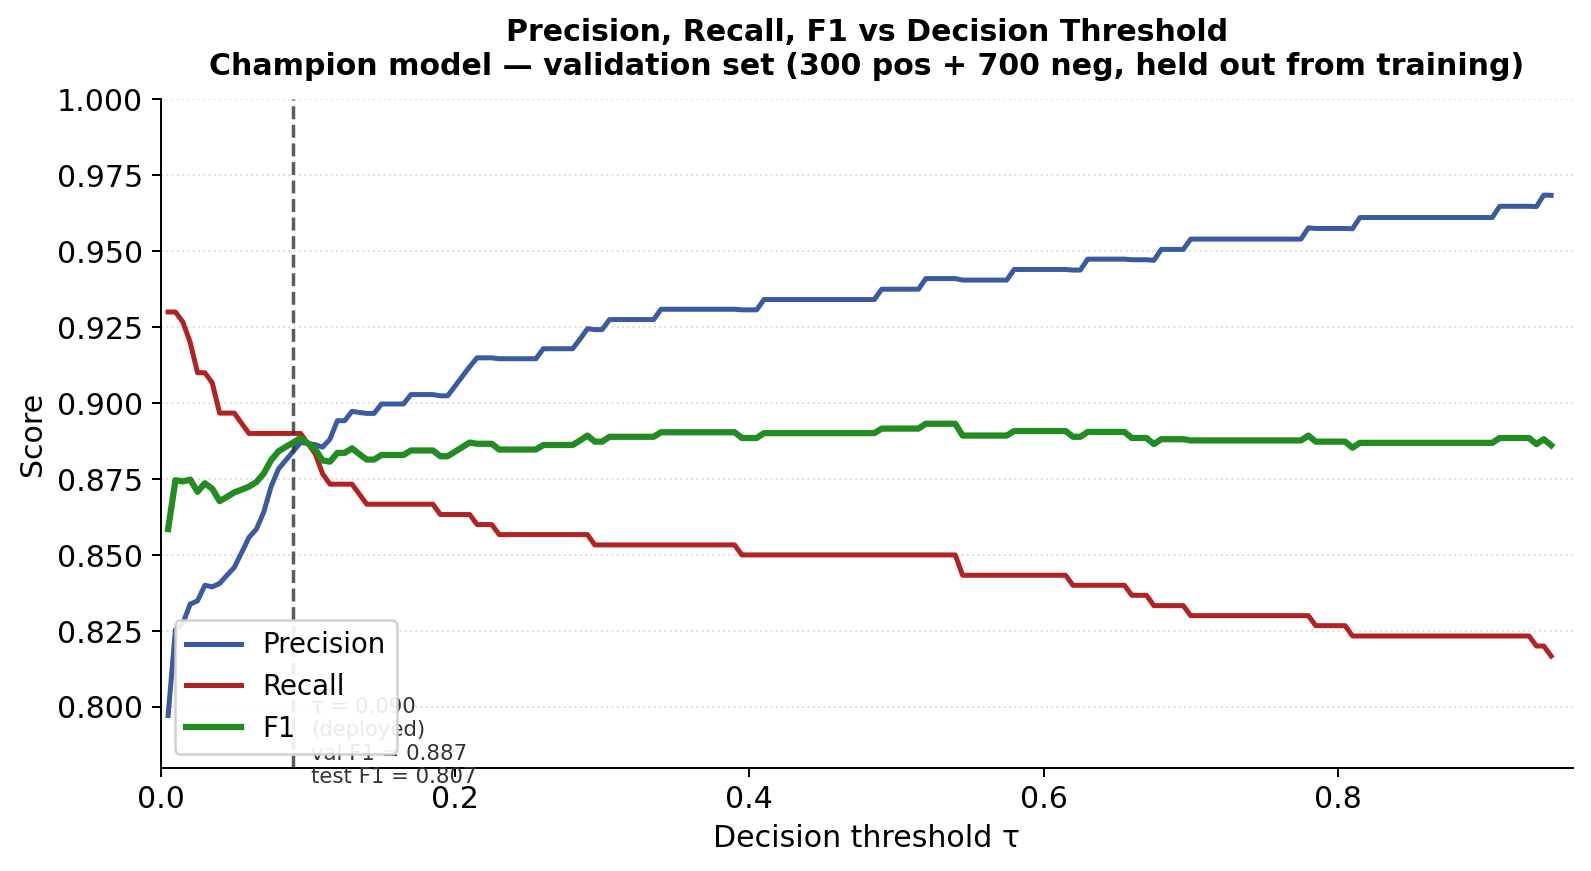
\includegraphics[width=0.6\textwidth]{fig_threshold_curve}
    \caption{Precision, recall, and F1 versus decision threshold on a
    300\,positive + 700\,negative held-out validation split (not seen
    during training) for an earlier cold-start checkpoint, illustrating
    threshold-curve shape rather than the currently-reported operating
    points. The annotated threshold $\tau{=}0.090$ achieves F1\,=\,0.887
    on this validation split. The currently-reported champion
    (Table~\ref{tab:main_results}) uses $\tau{=}0.360$, derived from its
    own 15\% held-out validation split, achieving test F1\,=\,0.874.}
    \label{fig:threshold}
\end{figure}

Both champions assign soft probabilities via knowledge distillation:
genuine interactions score predominantly in the range 0.2--0.6 rather
than near 1.0. For the checkpoint shown, F1 is nearly flat across
$\tau \approx 0.09$--$0.92$ on the validation split (0.887--0.893),
confirming that threshold selection is robust.

For applications where false positives entering a knowledge base are costly,
operating at higher $\tau$ increases precision at the cost of recall.
For the cold-start ablation: P\,=\,0.885, R\,=\,0.790 at $\tau{=}0.140$.
For the warm-start champion (P\,=\,0.925, R\,=\,0.829 at $\tau{=}0.360$),
raising $\tau$ further prioritises precision over recall analogously.
The threshold curves make these trade-offs explicitly visible and allow
practitioners to choose the operating point appropriate to their downstream
task.

\section{Test Set Integrity Details}
\label{app:contamination}

This appendix gives the full methodology behind the summary in
Section~\ref{sec:contamination}: three checks between the test set and
every training corpus used to produce a reported model.

\paragraph{Exact-match.} Comparing normalised (lower-cased,
whitespace- and punctuation-collapsed) test sentences against the
44,178-sentence distillation corpus (champion training data) and the
25,081-sentence template corpus (single-task baseline training data)
yields zero exact matches in both cases. Against the broader
34,880-sentence corpus used only for the teacher-chain analysis in
Section~\ref{sec:discussion} (not used to train any reported model),
exactly one test sentence is also present, originating from a
SIBiLS-harvested source. This same exact-match procedure additionally
uncovered that the eval-100 and BioTx-random sources, nominally
independent, share 96 of 100 sentences as the same underlying content
exported in two formats; they are merged into a single deduplicated
source (Section~\ref{sec:eval}) rather than double-counted. The 97
gen-set-150-extension sentences added to restore the test set to 500
were authored fresh for this evaluation and are by construction absent
from all training corpora.

\paragraph{Near-duplicate.} Using TF-IDF character $n$-gram
(3--5) cosine similarity with a threshold of 0.85, no additional
near-duplicates are found beyond the single exact match identified above.

\paragraph{Taxon-pair leakage.} The three GloBI-seeded test sources
(EP-A, EP-passage, BioTx-random) are seeded from specific taxon pairs;
even where the exact sentence differs, the same pair could also seed a
training template, constituting a subtler form of leakage. Comparing
each source's 100 taxon pairs against the template corpus's pairs
shows overlap of 1\% (EP-A), 1\% (EP-passage), and 0\% (BioTx-random).

\section{Extended Discussion: Architecture Figures and Downstream Utility}
\label{app:extended_discussion}

\begin{figure}[!ht]
    \centering
    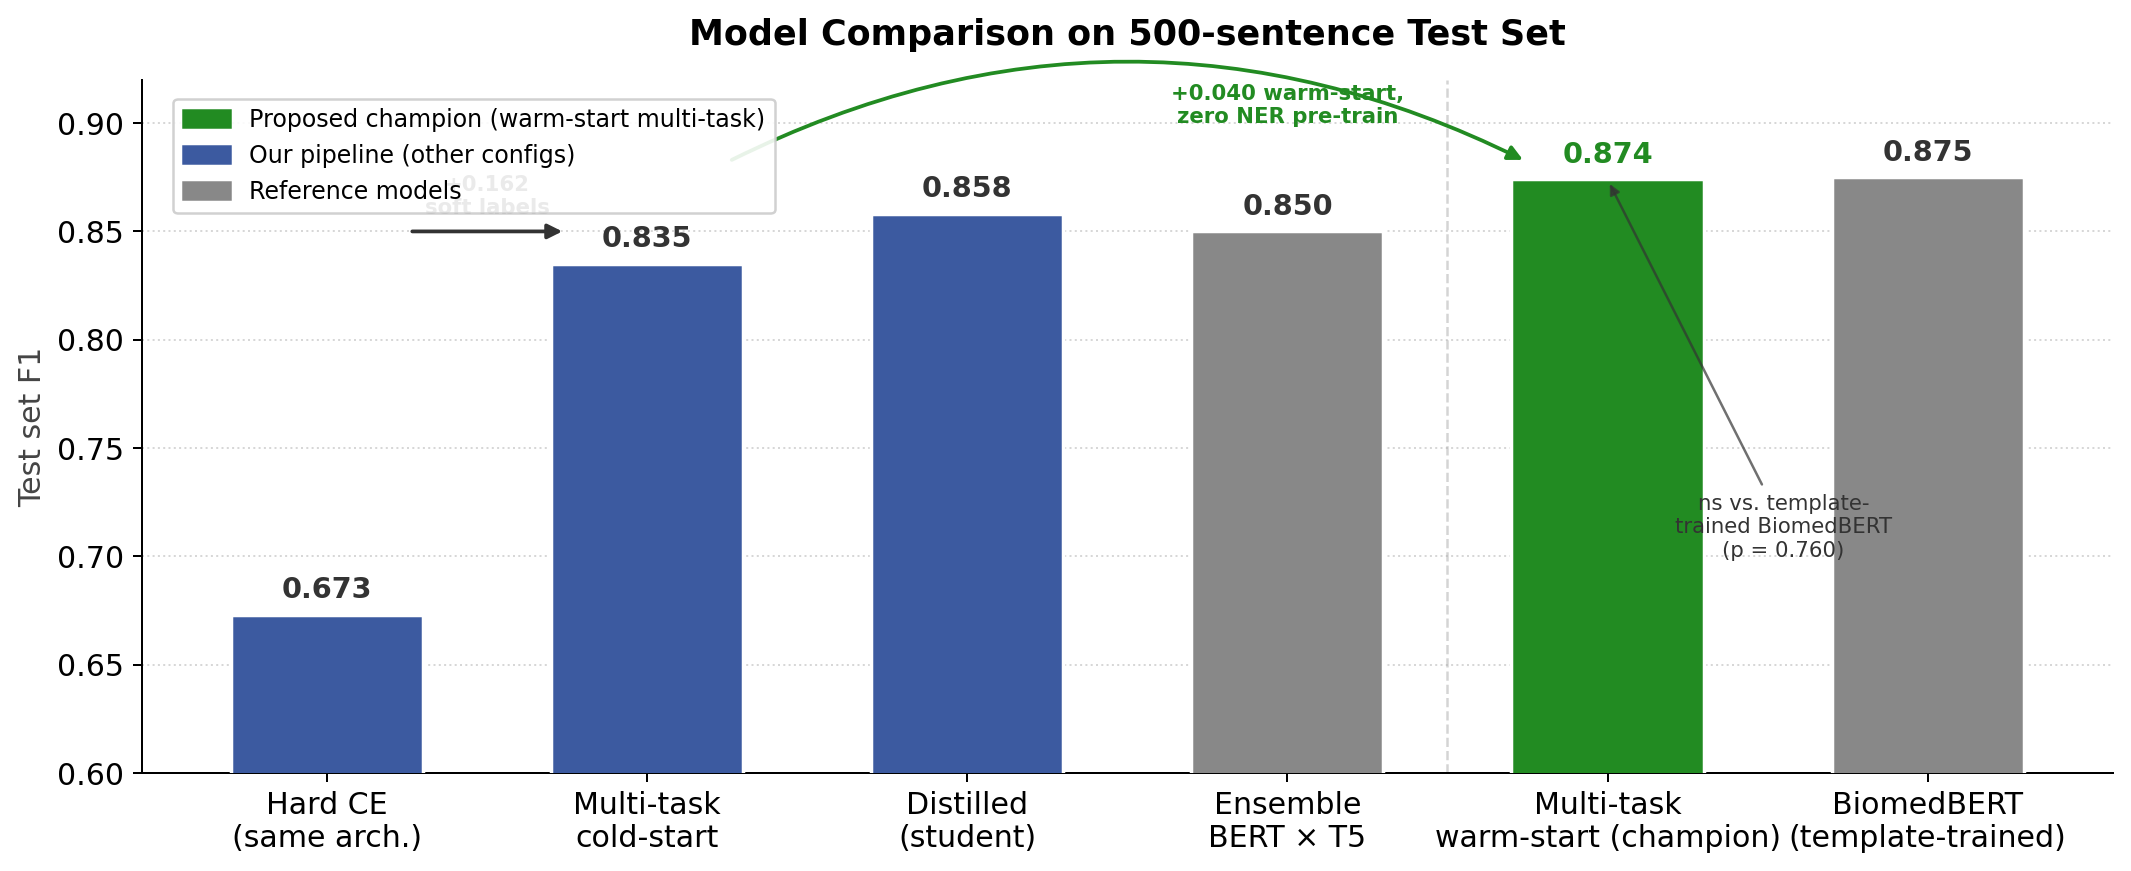
\includegraphics[width=0.7\textwidth]{fig_02_model_evolution}
    \caption{Test F1 across model architecture stages (numerically in
    Table~\ref{tab:main_results}). Annotated arrows
    indicate the primary driver of each improvement.}
    \label{fig:model_evolution}
\end{figure}

\begin{figure}[!ht]
    \centering
    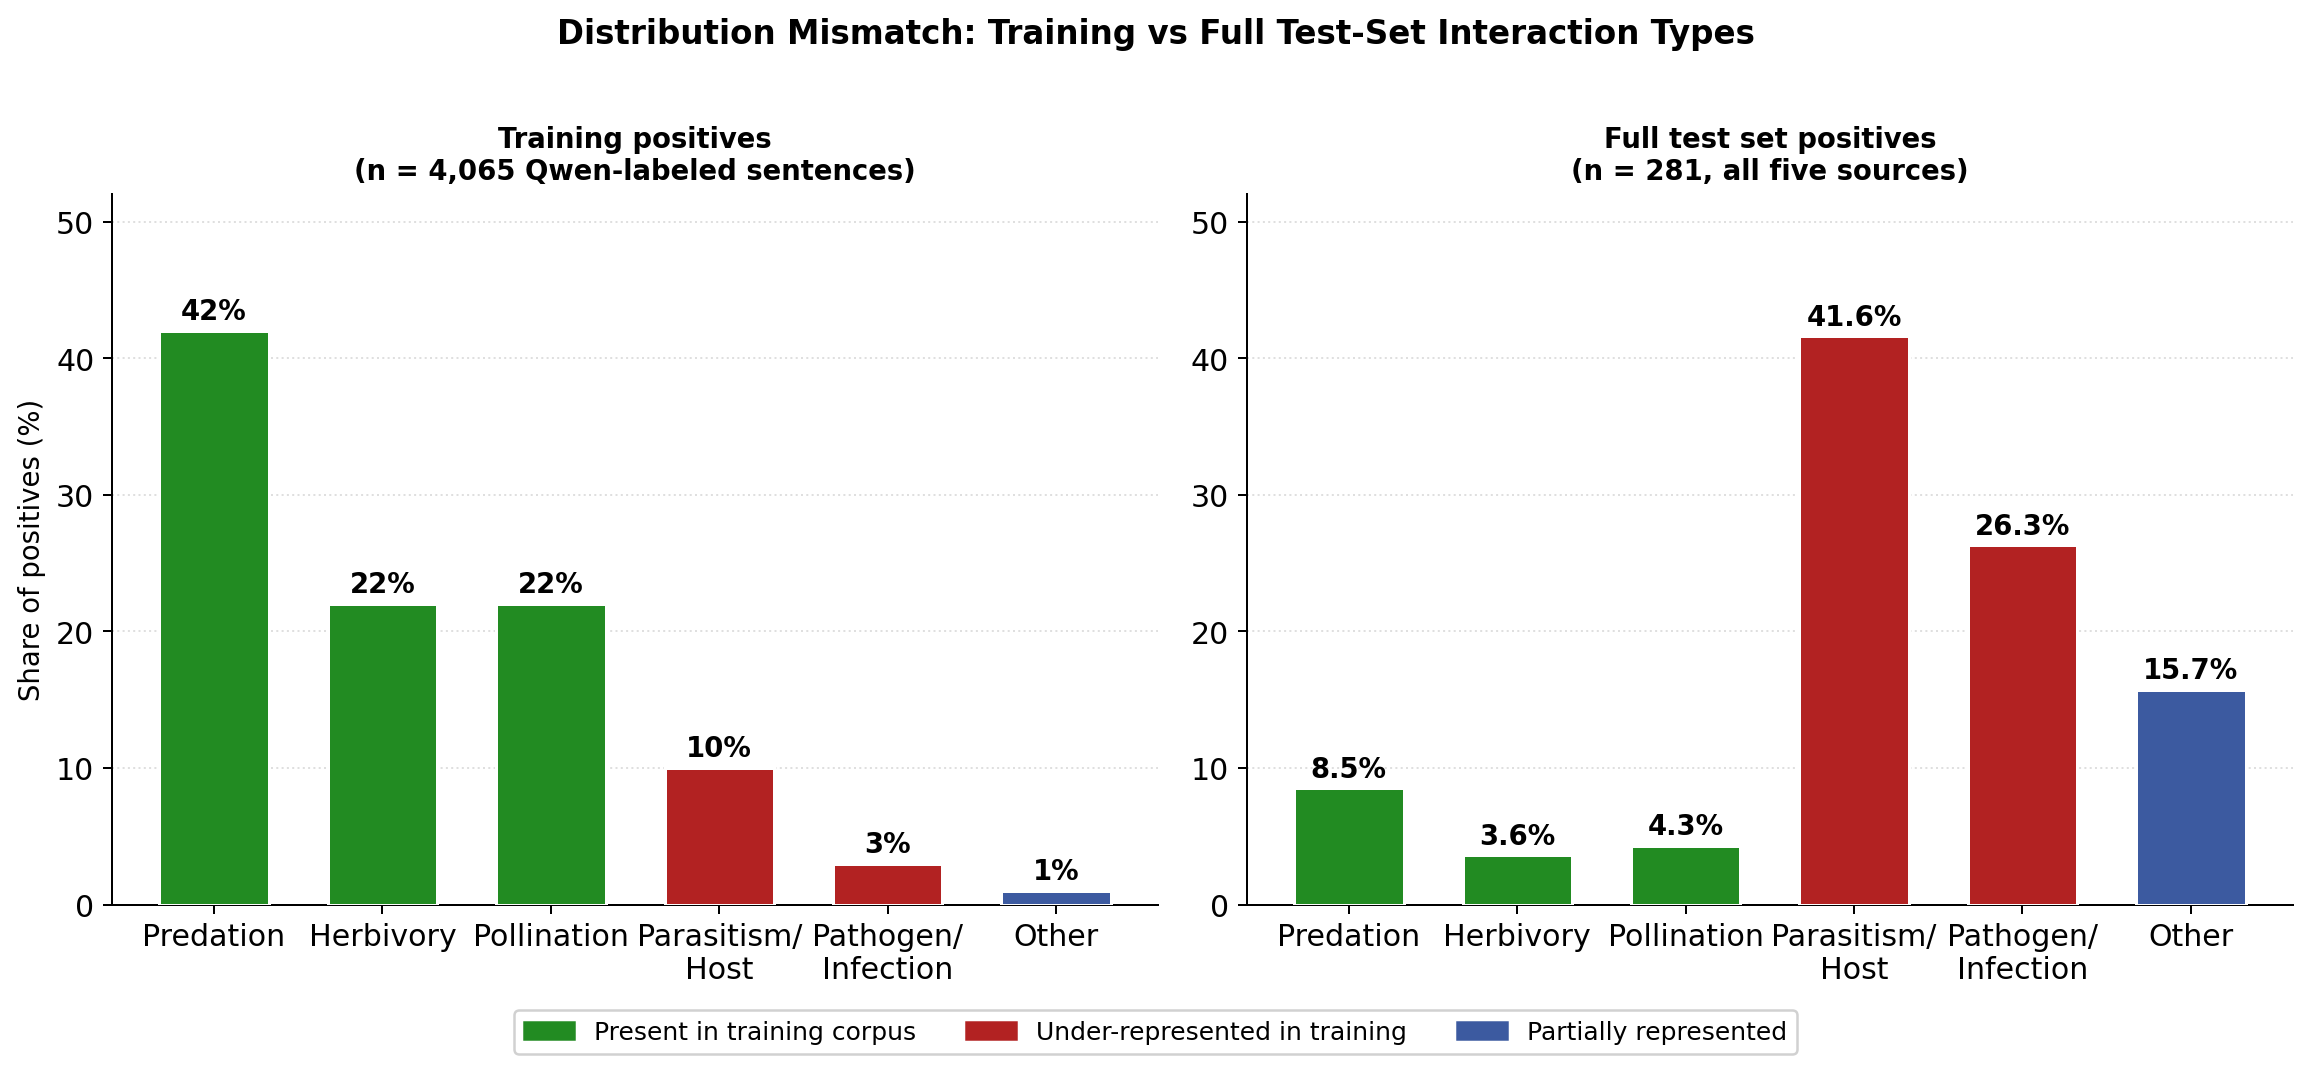
\includegraphics[width=0.85\textwidth]{fig_distribution_mismatch}
    \caption{Distribution of interaction types in training positives (left,
    n=4,065 Qwen-labeled sentences) versus the full test set's positives
    (right, n=281, aggregated across all five annotation sources).
    Categories are classified from GloBI interaction terms (EP-A,
    EP-passage, BioTx-random/eval-100) and the category field of
    gen-set-100 and gen-set-150-extension.
    Colors match between panels to highlight the same categories.}
    \label{fig:distribution}
\end{figure}

\subsection{Utility for BiotXplorer and Knowledge Graph Construction}

The classifier provides two concrete operational benefits for BiotXplorer.
First, as an upstream filter, it eliminates sentences that merely co-mention
taxa without describing an interaction, reducing index noise and improving
search relevance. Second, the calibrated probability output allows the
BiotXplorer platform to rank results by interaction confidence rather than
simple keyword match, enabling more nuanced retrieval.

For downstream knowledge graph construction, the multi-task model's NER
labels provide additional structure: the HOST/PATHOGEN
distinction produced by the NER head directly encodes the direction of the
knowledge graph edge (who interacts with whom), enabling the downstream
relation extractor to assign typed edges rather than undirected links.
This is particularly relevant for pathogen-host and parasite-host pairs
where edge direction is biologically meaningful.

\end{document}
